\documentclass{article}

\usepackage{float}
\usepackage{graphicx}
\usepackage{hyperref}

\title{App to Download Data from BACEN's API}
\author{Bernardo Paulsen}

\begin{document}

\maketitle

\section{Introduction}

An app was implemented to downoad time series data from Central Bank of Brazil's Time Series Management System.

\section{App}

The app gets the number of the series in BACEN's SGS (Sistema Gerenciador de Séries Temporais do Banco Central do Brasil), the start date and end date. It returns the time series in a dataframe.

\section{Test}

We test the app with the DI (Interbank Deposits) rate, which is number 12 on the Time Series Management System, and with the exchange rate (BRL/USD), which is number 1.

\begin{figure}[H]
	\caption{DI Rate}
	\centering
	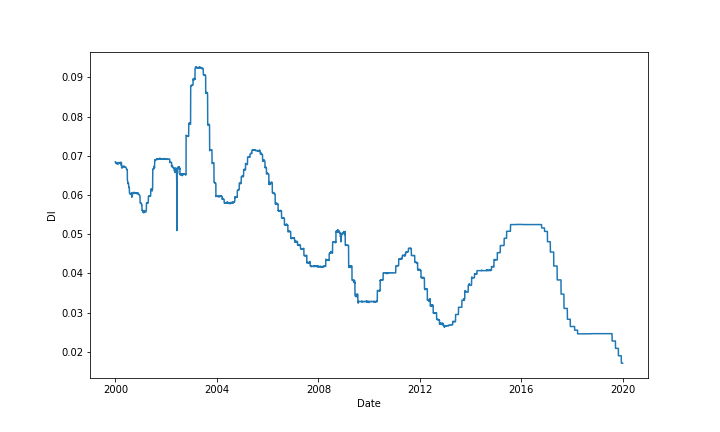
\includegraphics[width=\textwidth]{di.png}
\end{figure}


\begin{figure}[H]
	\caption{Exchange Rate}
	\centering
	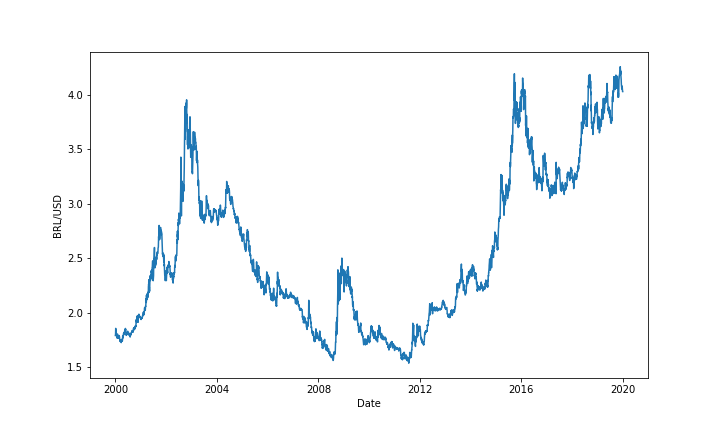
\includegraphics[width=\textwidth]{dol.png}
\end{figure}

\end{document}